\documentclass[12pt]{article}
% PACKAGE IMPORTS ----------------------------------------------
\usepackage{geometry}
\usepackage{titling}
\usepackage{enumitem}
\usepackage{ragged2e}
\usepackage{listings}
\usepackage{graphicx}
\usepackage{booktabs}
\usepackage{hyperref}
\usepackage{amsmath}

% FONT SELECTION -----------------------------------------------
\usepackage{tgschola}

% DOCUMENT CONFIGURATION ---------------------------------------
\geometry{letterpaper, margin = 1in}

\pretitle{\noindent \thickrule \skipsmall \centering \bfseries \Huge}
\posttitle{\skipsmall}
\preauthor{\centering \Large}
\postauthor{\skipsmall}
\predate{\centering \Large}
\postdate{\skipsmall \thickrule}

\setlist[enumerate,1]{label=\textbf{\Alph*.}, left = 0.5em, labelsep = 1em}

\lstset{inputencoding=utf8,language=C}
\lstdefinestyle{normal}{basicstyle=\ttfamily\small,breaklines=true,breakatwhitespace=true}
\lstdefinestyle{standalone}{frame=single,numbers=left,basicstyle=\ttfamily\footnotesize,breaklines=true,tabsize=2}

\hypersetup{hidelinks}

\author{Malcolm Riley}

% COMMAND DEFINITIONS ------------------------------------------
\newcommand{\skipsmall}{\vskip 0.5em}
\newcommand{\thickrule}{\rule{\textwidth}{2pt}}
\newcommand{\preparetitle}[1]{\title{Writeup: Homework \##1}}
\setlength{\droptitle}{-30pt}

\newcommand{\code}[1]{\texttt{#1}}
\newcommand{\codesingle}[1]{\begin{center}\fbox{\begin{minipage}{0.85\linewidth}\ttfamily#1\end{minipage}}\end{center}}
\newcommand{\codesample}[1]{\begin{center}\fbox{\begin{minipage}{0.85\linewidth}\lstinputlisting[style=standalone]{#1} \vspace{1em} \centering $\downarrow$ \par \vspace{1em} \input{#1} \\ \vspace{0.5em} \end{minipage}}\end{center}}

\newcommand{\tablehead}[1]{\toprule[2pt]#1\\ \toprule[2pt] \endhead}
\newcommand{\tablefoot}{\bottomrule[2pt]}

\newcommand{\quotes}[1]{``#1''}

\newcommand{\makesection}[2]{\newpage\section*{#1.\quad #2}}
\newcommand{\repolink}{https://github.com/malcolmriley/CMPM-163/blob/master/homework/Assets}
\newcommand{\shaderlink}[1]{\href{\repolink/Shaders/#1.shader}{\texttt{#1.shader}}}
\newcommand{\codelink}[1]{\href{\repolink/Scripts/#1.cs}{\texttt{#1.cs}}}

\preparetitle{2}

\begin{document}
\maketitle

\section*{Introduction}
As with the previous assignment, all subtasks of this assignment have been implemented as a single Unity Scene. No third-party Unity packages were used to create this scene. All code and scene assets including models and sounds were created by myself for the purpose of this assignment.

The controls necessary for interacting with the scene are depicted onscreen, but the mouse can be used to look in a particular direction, and the shift key can be pressed to zoom towards the vehicle and slow time.

\makesection{A}{Tron Filter}
\begin{center}
	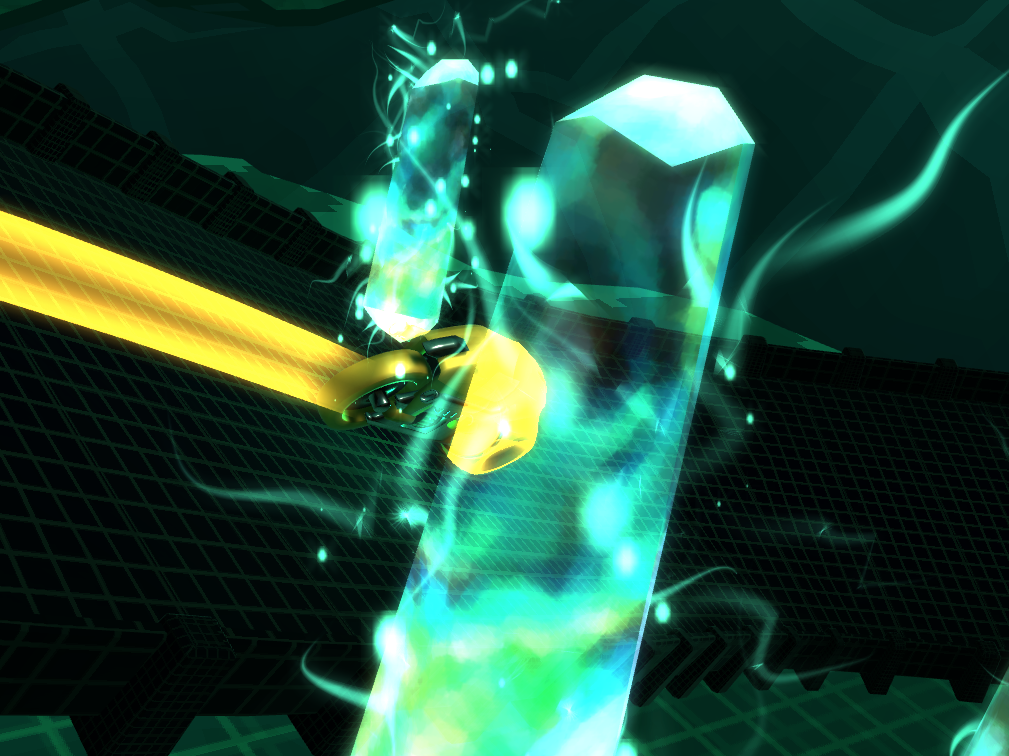
\includegraphics[width=0.5\linewidth]{part1.png}
\end{center}
\subsection*{Bloom Filter}
To implement the bloom filter, I created a second \quotes{VFX Camera} object. This camera's culling mask is set so that it only draws objects on the \quotes{Transparent FX} render layer, and the main camera is set to not render objects on that layer. The \quotes{VFX Camera} is furthermore configured to output to an intermediate \code{RenderTexture}. This \code{RenderTexture} is subsequently blended additively to the main scene render in the \code{CameraVFX} class, via the \code{CameraVFXBloon} shader. This shader performs a simple iterative box blur on the \code{RenderTexture} derived from the \quotes{Transparent FX} layer, adding the result to the primary lookup and main texture.

While this approach does not use emission properties in any way, a benefit is that it is trivially easy to add bloom to a particular object: simply switch the object's render layer to \quotes{Transparent FX}. An obvious shortcoming is that since the \quotes{Transparent FX} layer is additively blended to the main scene, objects on this layer will appear transparent and emissive, and will not be properly occluded by main scene geometry (since a separate depth buffer is used for each camera's render target). These shortcomings were acceptable in the limited case of this assignment.

\subsection*{Rim Shader}
The rim shader was implemented as a custom material applied to the desired mesh. The result was achieved via the simple dot product of the world space normal and world space view vector, multiplied by the desired color and an arbitrary intensity factor.

To achieve the extra credit requirement, the stencil buffer was employed in the \code{GlowOverlay} and \code{VFXOccluder} shaders. While admittedly, the name is a bit of a misnomer, the stencil operation in the \code{VFXOccluder} shader permits the \code{GlowOverlay} render to persist whenever the two meshes occupy the same screen space, and the \code{VFXOccluder}-rendered mesh is in front of the \code{GlowOverlay}-enabled mesh.

\subsection*{Links}
Camera VFX Adder: \codelink{CameraVFX}\\
Bloom Material Shader: \shaderlink{CameraVFXBloon}
Rim Shader: \shaderlink{GlowOverlay}\\
Rim Shader Complement Occluder: \shaderlink{VFXOccluder}

\makesection{B}{Outdoor 3D Scene}
\begin{center}
	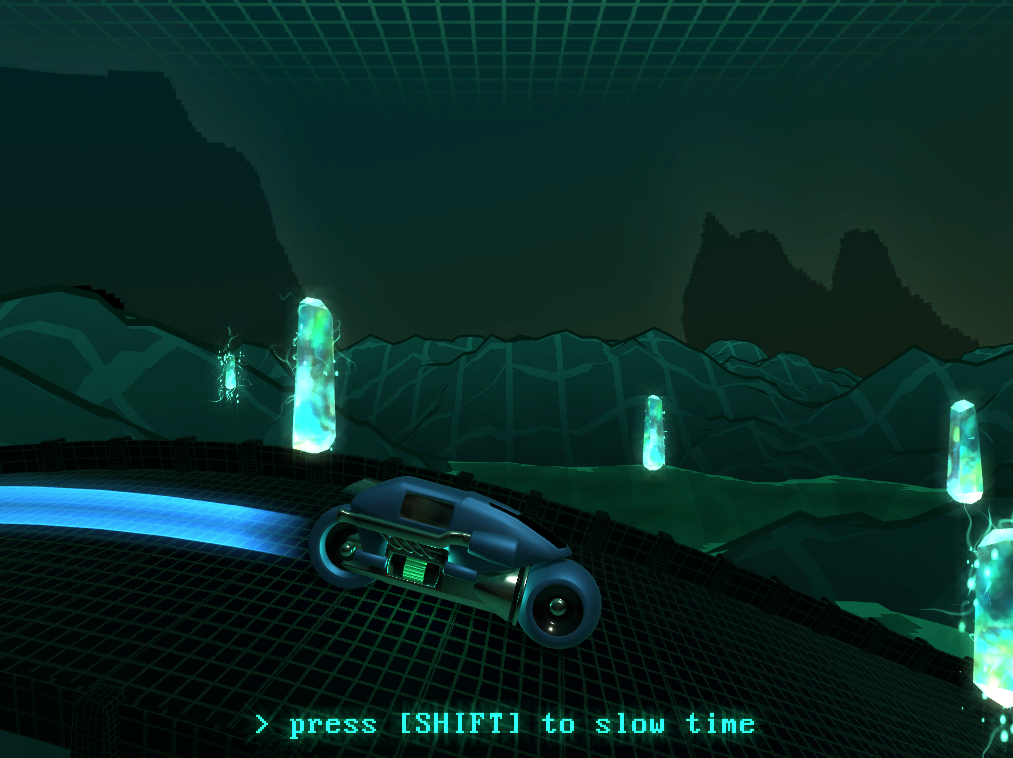
\includegraphics[width=0.5\linewidth]{part2.png}
\end{center}

\subsection*{Height Map}
The terrain heightmap deformation was implemented as a vertex-displacement shader applied to a flat plane mesh. This shader samples the red channel from an arbitrary image, and offsets the vertex by this channel value times an arbitrary \quotes{Height} property.

\subsection*{Water}
The water shader samples the skybox cubemap in order to give the appearance of reflecting the sky. To produce the pixelated \quotes{edge foam} effect, the shader samples from the same heightmap texture as the terrain -- beyond the threshold \quotes{Height} property, the water fragment shader draws a lighter color. This threshold is varied slightly over time for a subtle motion effect.

Although the shader does not technically meet the extra-credit requirement of refracting objects \textit{beneath} the water's surface, the shader does employ the \code{refract()} function add limited apparent motion to the water surface.

\subsection*{Links}
Heightmap Mesh Deformation Shader: \shaderlink{TerrainDisplace}\\
Cubemap-Reflecting/Refracting Water Shader: \shaderlink{WaterShader}

\end{document}